\documentclass[11pt, a4paper]{article}
\usepackage[utf8]{inputenc}
\usepackage{fontenc}
\usepackage{geometry}
\usepackage{graphicx}
\usepackage{tikz}
\usepackage{amsmath}
\usepackage{amssymb}
\usepackage{fancyhdr}
\usepackage{enumitem}
\usepackage{booktabs}
\usepackage{caption}
\usepackage{subcaption}
\usepackage{float} % Allow [H] placement to keep figures in place

% Page Geometry
\geometry{left=25mm, right=25mm, top=25mm, bottom=25mm}


% Header and Footer configuration
\pagestyle{fancy}
\fancyhf{}
\lhead{\textbf{R\&IA ‒ AI352}}
\rhead{Assignment 01: Robot Anatomy \& Terminologies}
\cfoot{\thepage}
\renewcommand{\headrulewidth}{1pt}

% TikZ Libraries for Schematics
\usetikzlibrary{shapes, arrows.meta, calc, positioning, patterns, decorations.pathmorphing}

\newcommand{\horrule}[1]{\rule{\linewidth}{#1}} % Create horizontal rule command with 1 argument of height

\title{	
\normalfont \normalsize 
\textsc{Robotics and its Application (AI352) | Assignment 2} \\ [25pt] % Your university, school and/or department name(s)
\huge Robot Anatomy and Terminologies \\ % The assignment title
\horrule{2pt} \\[0.5cm] % Thick bottom horizontal rule
}

\author{U23CS014 | Naishadh Rana} % Your name
\date{}

\begin{document}

\maketitle % Print the title

\section*{Part A: Robot Anatomy}

\subsection*{1. Identify Robot Components}
For each robot listed below, examine the provided schematic, label the indicated components, and analyze the kinematic structure.

% --- MOVEMASTER RM-501 SCHEMATIC ---
\begin{figure}[h]
    \centering
    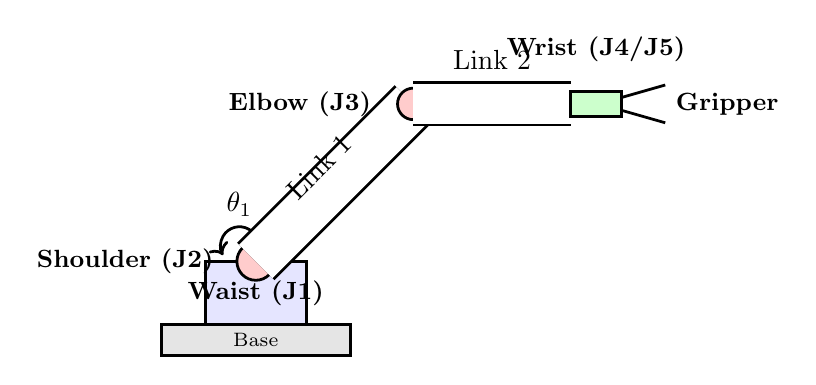
\begin{tikzpicture}[scale=0.8, line width=1pt]
        % Base
        \fill[gray!20] (-1.5,0) rectangle (1.5,0.5);
        \draw (-1.5,0) -- (1.5,0) -- (1.5,0.5) -- (-1.5,0.5) -- cycle;
        \node at (0,0.25) {\scriptsize Base};
        
        % Waist (J1)
        \draw[fill=blue!10] (-0.8,0.5) rectangle (0.8,1.5);
        \node at (0,1) {\small \textbf{Waist (J1)}};
        \draw[->] (0,1.6) arc (-30:210:0.3) node[midway, above] {$\theta_1$};

        % Shoulder (J2)
        \draw[fill=red!20] (0,1.5) circle (0.3);
        \node[left=0.4cm] at (0,1.5) {\small \textbf{Shoulder (J2)}};
        
        % Link 1 (Upper Arm)
        \draw[double, double distance=6mm] (0,1.5) -- (2.5,4);
        \node[rotate=45] at (1,3) {Link 1};

        % Elbow (J3)
        \draw[fill=red!20] (2.5,4) circle (0.25);
        \node[left=0.4cm] at (2.5,4) {\small \textbf{Elbow (J3)}};

        % Link 2 (Forearm)
        \draw[double, double distance=5mm] (2.5,4) -- (5,4);
        \node[above=3mm] at (3.75,4) {Link 2};

        % Wrist Assembly (Differential)
        \draw[fill=green!20] (5,3.8) rectangle (5.8,4.2);
        \node[above=4mm] at (5.4,4) {\small \textbf{Wrist (J4/J5)}};
        
        % End Effector
        \draw (5.8,4.1) -- (6.5,4.3);
        \draw (5.8,3.9) -- (6.5,3.7);
        \node[right] at (6.5,4) {\small \textbf{Gripper}};
        
    \end{tikzpicture}
    \caption{\textbf{Movemaster RM-501}: A 5-DOF educational manipulator. Note the differential wrist mechanism at the distal end of Link 2.}
    \label{fig:rm501}
\end{figure}

% --- PUMA 560 SCHEMATIC ---
\begin{figure}[h]
    \centering
    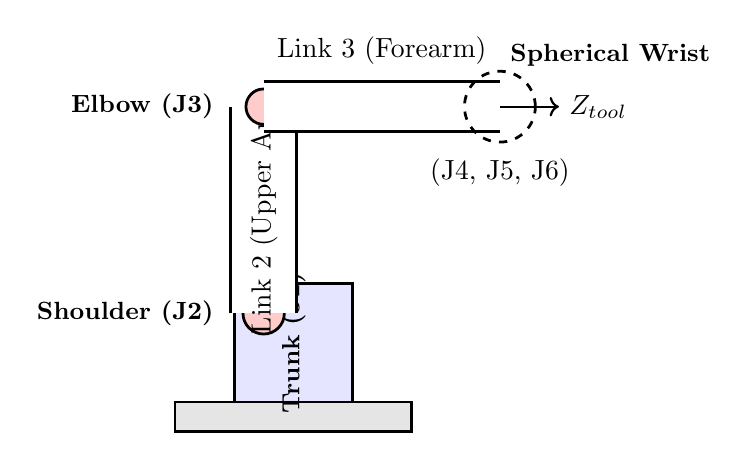
\begin{tikzpicture}[scale=0.75, line width=1pt]
        % Base
        \fill[gray!20] (-2,0) rectangle (2,0.5);
        \draw (-2,0) -- (2,0) -- (2,0.5) -- (-2,0.5) -- cycle;
        
        % Trunk (J1)
        \draw[fill=blue!10] (-1,0.5) rectangle (1,2.5);
        \node[rotate=90] at (0,1.5) {\small \textbf{Trunk (J1)}};

        % Shoulder (J2) - Note Offset
        \draw[fill=red!20] (-0.5,2.0) circle (0.35);
        \node[left=0.5cm] at (-0.5,2.0) {\small \textbf{Shoulder (J2)}};
        
        % Link 2 (Upper Arm)
        \draw[double, double distance=8mm] (-0.5,2.0) -- (-0.5,5.5);
        \node[rotate=90] at (-0.5,3.75) {Link 2 (Upper Arm)};

        % Elbow (J3)
        \draw[fill=red!20] (-0.5,5.5) circle (0.3);
        \node[left=0.5cm] at (-0.5,5.5) {\small \textbf{Elbow (J3)}};

        % Link 3 (Forearm)
        \draw[double, double distance=6mm] (-0.5,5.5) -- (3.5,5.5);
        \node[above=4mm] at (1.5,5.5) {Link 3 (Forearm)};

        % Spherical Wrist
        \draw[dashed] (3.5,5.5) circle (0.6);
        \node[above right] at (3.5,6) {\small \textbf{Spherical Wrist}};
        \node[below] at (3.5,4.8) {(J4, J5, J6)};
        
        % Flange
        \draw[->, thick] (3.5,5.5) -- (4.5,5.5) node[right] {$Z_{tool}$};

    \end{tikzpicture}
    \caption{\textbf{PUMA 560}: A 6-DOF research manipulator featuring a spherical wrist and shoulder/elbow offsets.}
    \label{fig:puma560}
\end{figure}

% --- KGP-50 SCHEMATIC ---
\begin{figure}[h]
    \centering
    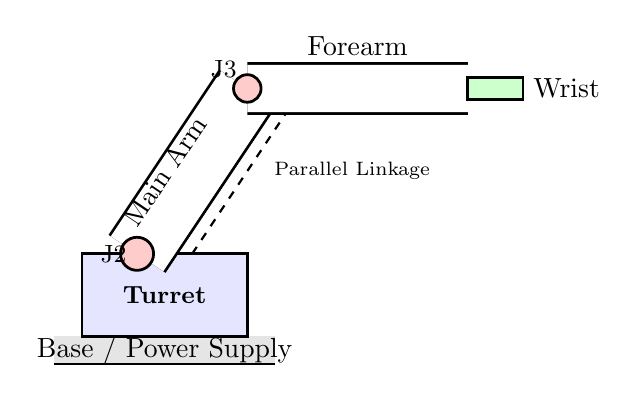
\begin{tikzpicture}[scale=0.7, line width=1pt]
        % Base
        \fill[gray!20] (-2,0) rectangle (2,0.5);
        \draw (-2,0) -- (2,0);
        \node at (0,0.25) {Base / Power Supply};

        % Turret
        \draw[fill=blue!10] (-1.5,0.5) rectangle (1.5,2.0);
        \node at (0,1.25) {\small \textbf{Turret}};

        % Parallel Linkage Mechanism
        \coordinate (J2) at (-0.5, 2.0);
        \coordinate (J3) at (1.5, 5.0);
        \coordinate (MotorJ3) at (0.5, 2.0); % Conceptual motor mount
        \coordinate (LinkPoint) at (2.5, 5.0);
        
        % Main Lift Arm
        \draw[double, double distance=8mm, fill=white] (J2) -- (J3);
        \node[rotate=56] at (0, 3.5) {Main Arm};
        \draw[fill=red!20] (J2) circle (0.3);
        \node[left] at (J2) {\small J2};

        % Parallel Bar (Simulating the closed chain)
        \draw[dashed, thick] (MotorJ3) -- (LinkPoint);
        \draw[dashed, thick] (J3) -- (LinkPoint);
        \node[right] at (1.8, 3.5) {\scriptsize Parallel Linkage};

        % Forearm
        \draw[double, double distance=6mm, fill=white] (J3) -- (5.5, 5.0);
        \node[above] at (3.5, 5.4) {Forearm};
        \draw[fill=red!20] (J3) circle (0.25);
        \node[above left] at (J3) {\small J3};

        % Wrist
        \draw[fill=green!20] (5.5, 4.8) rectangle (6.5, 5.2);
        \node[right] at (6.5, 5.0) {Wrist};

    \end{tikzpicture}
    \caption{\textbf{KGP-50}: A high-payload industrial prototype utilizing a parallel linkage structure for the primary lifting axes.}
    \label{fig:kgp50}
\end{figure}

\newpage

\subsection*{2. Component Definitions and Functions}
Based on the diagrams above, define the following core components:

\begin{enumerate}
    \item \textbf{Manipulator:} The mechanical structure consisting of rigid links and movable joints. \textit{Function:} Provides the physical reach and structural integrity to position the end-effector.
    \item \textbf{Joints:} Kinematic pairs (Revolute or Prismatic). \textit{Function:} Constrain motion to a single Degree of Freedom (DOF), enabling controlled articulation.
    \item \textbf{Links:} Rigid members connecting joints. \textit{Function:} Determine the workspace geometry (reach) and transmit forces.
    \item \textbf{End-Effector:} The tool attached to the robot flange. \textit{Function:} Interacts with the environment (e.g., Gripper, Welding Torch).
    \item \textbf{Power Supply:} Energy conversion unit. \textit{Function:} Converts AC facility power to regulated DC/AC bus voltages for actuators and logic circuits.
    \item \textbf{Controller:} Computational unit (DSP/Microprocessor). \textit{Function:} Solves kinematics, generates trajectories, and closes the servo control loops.
\end{enumerate}

\subsection*{3. Degrees of Freedom (DOF) Analysis}
For each robot, determine the DOF of the indicated joints and justify the classification:
\begin{table}[h]
    \centering
    \begin{tabular}{|l|c|p{8cm}|}
        \hline
        \textbf{Robot} & \textbf{Total DOF} & \textbf{Justification of Joints} \\
        \hline
        RM-501 & 5 & Joints 1-3 provide positioning (X,Y,Z). Joints 4-5 (Pitch/Roll) provide orientation but lack Yaw, preventing rotation about the vertical tool axis. All joints are Revolute. \\
        \hline
        PUMA 560 & 6 & Features 3 Revolute joints for positioning and a 3-DOF Spherical Wrist (Roll-Pitch-Roll) allowing arbitrary orientation in space. \\
        \hline
        KGP-50 & 6 & Uses a parallel linkage structure but functions as a 6-DOF articulated arm. The linkage couples the elbow motion to the shoulder but provides 6 independent control axes. \\
        \hline
    \end{tabular}
\end{table}

\section*{Part B: Simulation Instructions}

\begin{enumerate}
    \item \textbf{Input–Output Relationship:}
    \begin{itemize}
        \item Input: Joint angles $(\theta_1, \theta_2, \theta_3, \ldots)$
        \item Output: End-effector position (x, y, z) and orientation.
        \item Relation: Forward kinematics maps joint angles $\to$ position.
        \begin{figure}[H]
                \centering
                \includegraphics[width=0.25\linewidth]{init.png}
                \caption{Movemaster}
                \label{fig:placeholder}
        \end{figure}
        \end{itemize}
    
    \item \textbf{Workspace:}
    \begin{itemize}
        \item Definition: All points the end-effector can reach.
        \item Depends on: number of joints, link lengths, and joint limits.
        \item Practical step: generate $N=10{,}000$ random joint configurations within limits and plot the resulting 3D point cloud to reveal the work envelope and singular voids.
    \end{itemize}

    \item \textbf{Trajectory:}
    \begin{itemize}
        \item Definition: Path followed by the end-effector from start to target.
        \item Joint-space trajectory: interpolate in joint coordinates (curved tool path).
        \item Cartesian-space trajectory: interpolate in task space (straight-line tool path; requires inverse kinematics at each step).
    \end{itemize}

    \item \textbf{Motion Simulation:}
    \begin{itemize}
        \item Define start point $A$ and end point $B$ in joint space.
        \item Interpolate linearly between $A$ and $B$ over time $t$.
        \item Animate the link structure (stick figure) at each time step.
    \end{itemize}
    
    \item \textbf{Trajectory Tracing:}
    \begin{itemize}
        \item Record the end-effector tip position at every simulation step.
        \item Plot a continuous trace line to visualize the path.
        \item Compare joint-space vs. Cartesian-space interpolation traces.
    \end{itemize}
\end{enumerate}

\end{document}